\begin{pastexam}[label={px:ust-114-ee-ds-09}]{臺聯大電機類 114 學年度 第 9 題}
（單選；2 分，答錯不倒扣）

What is the height of a binary search tree after inserting 3, 41, 52, 26, 38, 57, 9, 49 sequentially?
The tree is empty initially.

(A)~1 \qquad (B)~2 \qquad (C)~3 \qquad (D)~4
\end{pastexam}

\begin{pastsoln}
答案是 (C)。 高度照前一題的定義，用邊數算。

依序插入（資結書虛擬碼~9.6，比節點小往左、否則往右）：
\begin{itemize}
\item 3 是根；41 $> 3$，接在 3 的右邊；52 $> 3$、$> 41$，接在 41 的右邊。
\item 26：$> 3$、$< 41$，接在 41 的左邊；38：$> 3$、$< 41$、$> 26$，接在 26 的右邊。
\item 57：一路往右，接在 52 的右邊；9：$> 3$、$< 41$、$< 26$，接在 26 的左邊。
\item 49：$> 3$、$> 41$、$< 52$，接在 52 的左邊。
\end{itemize}
\begin{center}
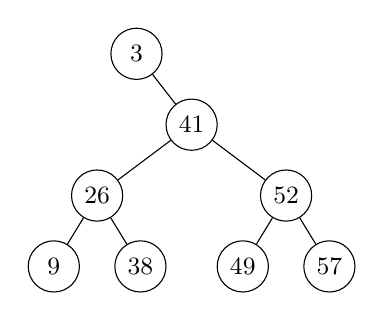
\begin{tikzpicture}[every node/.style={circle,draw,minimum size=6.5mm,inner sep=0pt,font=\small},
  level distance=9mm, level 1/.style={sibling distance=14mm}, level 2/.style={sibling distance=24mm},
  level 3/.style={sibling distance=11mm}]
\node {3} child[missing] child {node {41}
  child {node {26} child {node {9}} child {node {38}}}
  child {node {52} child {node {49}} child {node {57}}}};
\end{tikzpicture}
\end{center}
最深的節點 9、38、49、57 都在根下面 $3$ 條邊（例如 $3 \to 41 \to 26 \to 9$），高度 $3$。
(A)(B)(D) 都不對。
\end{pastsoln}
